\chapter{Metodología}
%\addcontentsline{toc}{chapter}{Metodología}



En la Figura \ref{metodologia} se presenta el esquema metodológico adoptado para la ejecución del proyecto, en el cual se pueden apreciar los principales elementos, ejes y fases que definen el desarrollo del proyecto de investigación.
\begin{figure}[ht]
\centering
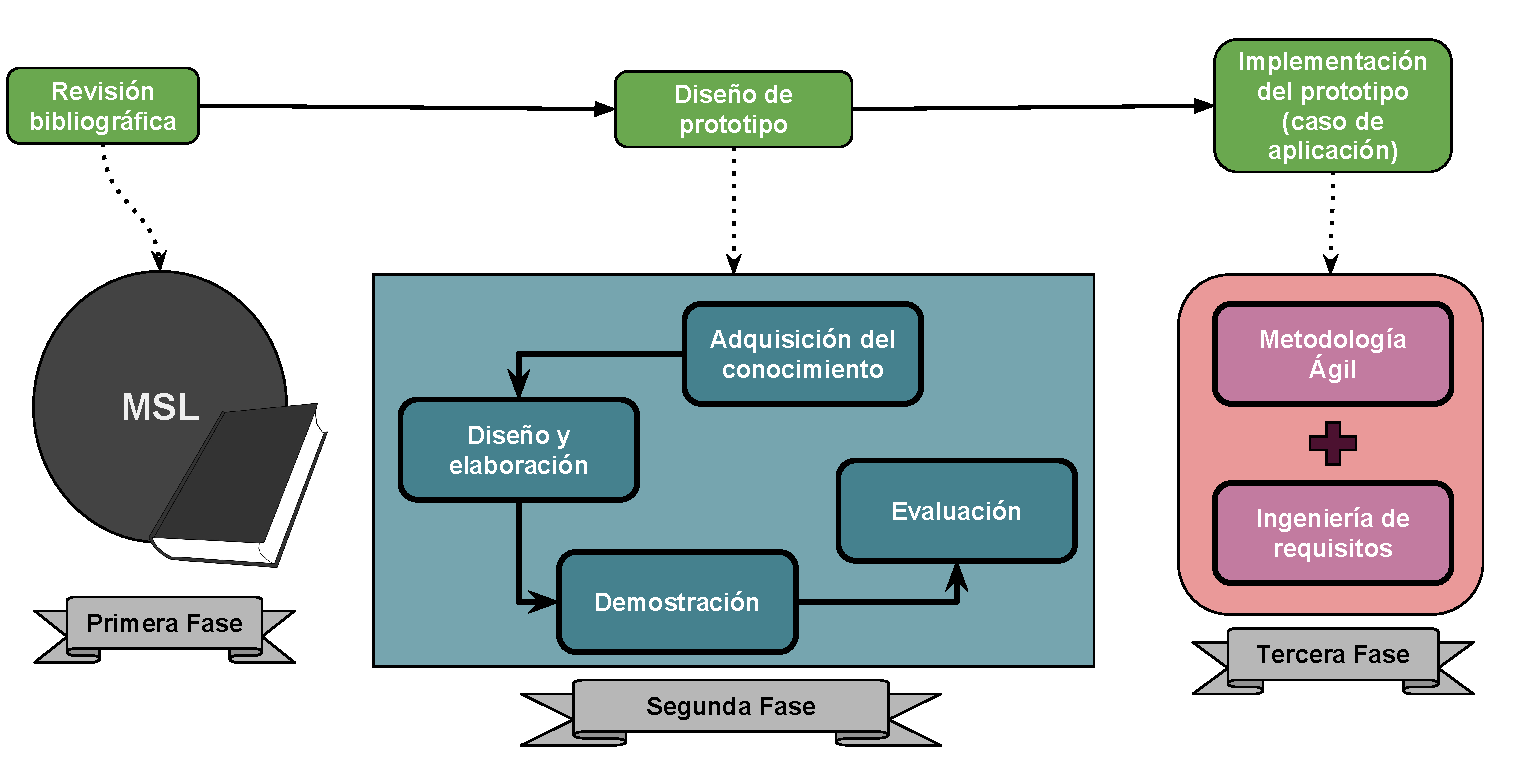
\includegraphics[width=16cm, height=8cm]{metodologia}
\caption{Metodología adoptada en el proyecto de investigación}
\label{metodologia}
\end{figure}


\begin{itemize}

\item \textbf{\textit{Primera fase:}} Con el fin de documentar las técnicas de minería de datos (MD) empleadas en la ingeniería de líneas de producto (ILP), se realizó una revisión de la literatura mediante la metodolgía \textit{Systematic Mapping Studies} (SMS por sus siglas en inglés) o mapeo sistemático de la literatura (MSL),  la cual consistió en categorizar y caracterizar un conjunto de documentos en diferentes dimensiones, mediante el  desarrollo de las etapas presentadas a continuación. Es de anotar que el proceso de MSL consiste en las cinco etapas posteriores a la planeación, ya que esta depende de cada investigador. 
%al usar estudios sistemáticos  se redujo el sesgo en la investigación \cite{Petersen2015}, el resultado fue un estudio completo y replicable. Con los hallazgos realizados, se pudo seleccionar más fácilmente las técnicas de minería de datos que se aplicaron en la elaboración de los modelos de características.El SMS presento un conjunto de documentos caracterizados y categorizados en una gran cantidad de dimensiones y características que consta de 5 etapas: 

\begin{enumerate}
\item En la primera etapa se realiza la planeación de la revisión.
\item En la segunda etapa se definieron las preguntas de investigación.
\item En la tercera etapa se ejecuto la búsqueda que daría respuesta a las preguntas planteadas anteriormente.
\item La cuarta etapa consistió en el escaneo de la bibliografía, el cual puede ser manual o automático.
\item La quinta etapa fue la clasificación de los estudios encontrados. 
\item La última etapa consistió en el mapeo de los datos encontrados, lo cual derivó en un documento llamado protocolo o informe final.
\end{enumerate}

\item \textbf{\textit{Segunda fase:}} En esta fase se construyeron los modelos de proceso y de producto aplicando un enfoque o filosofía basado en la metodología Design Science \cite{Vaishnavi2013} haciendo énfasis en el entendimiento de las diferentes capas en los sistemas de información. Posteriormente estos modelos fueron probados con el repositorios de datos \href{http://archive.ics.uci.edu/ml/datasets/Iris}{Iris}, con el propósito de construir un MC y, a partir de esta demostración, mejorar el método empleado.

\item \textbf{\textit{Tercera fase:}} En esta fase se dejó constancia de la implementación del método seleccionado, teniendo en cuenta la dificultad que se presentó por la gran cantidad de datos. En las etapas de implementación y pruebas del ciclo de desarrollo del software se incluyeron el agilismo, también llamado metodologías ágiles \cite{Alaimo2013}, y las tecnologías en la nube para un control permanente y continuo. El propósito de estas etapas consistió en un desarrollo incremental basado en objetivos simples y fáciles de alcanzar, cuyo control de cumplimiento se desarrolló mediante entregas al tutor o al grupo de investigación y, con sus correcciones, se realizaron paulatinamente los avances en el desarrollo.
El objetivo de esta fase fue un desarrollo de un código en plataformas abiertas que pueda ser usado por toda la comunidad académica.
\end{itemize}

\section{Revisión bibliográfica mediante mapeo sistemático de la literatura}

En esta sección se aplicaron las guías propuestas por Petersen, \textit{et al.} \cite{Petersen2008a} para el desarrollo del MSL. Sin embargo, a este proceso de mapeo que originalmente posee cinco etapas, le fue añadida una etapa previa de planeación de la revisión, como se muestra en la Figura \ref{sms}, donde puede observarse también que cada etapa posee un producto derivado, el cual se mostrará en el desarrollo del documento.
\newpage


\begin{figure}[h]
    \centering
    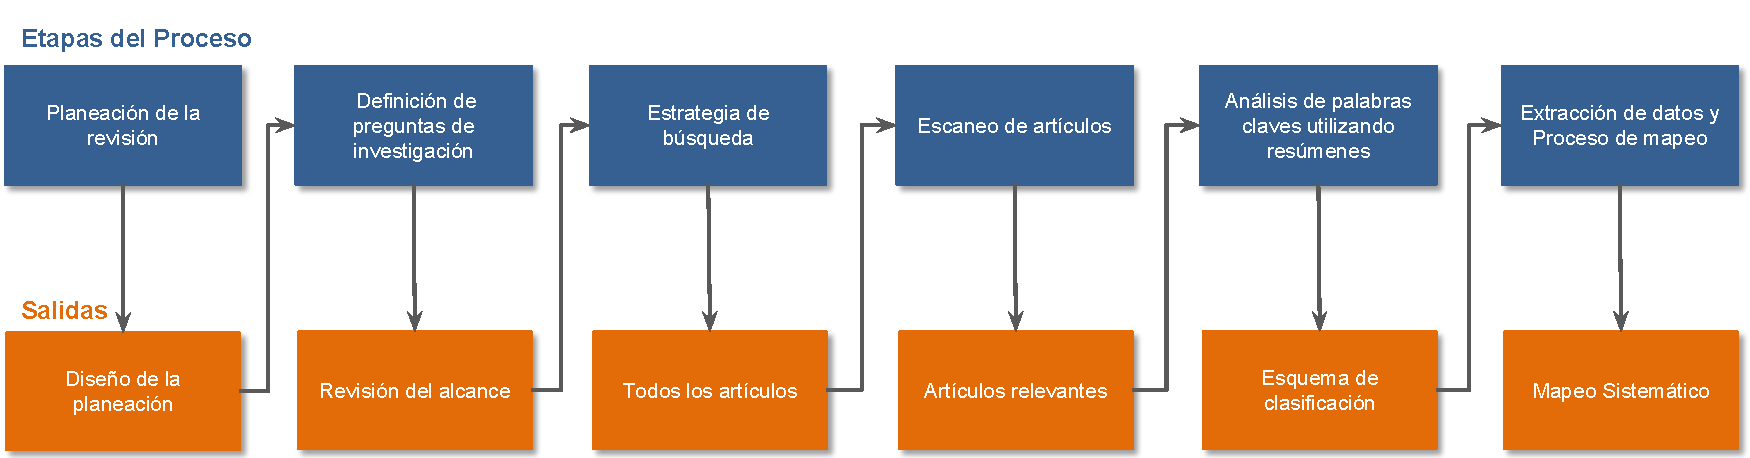
\includegraphics[width=0.9\textwidth]{sms}
    \caption{Mapeo Sistemático de la Literatura propuesto por Petersen,\textit{et al.}}
    \label{sms}
\end{figure}

\subsection{Planificación de la revisión}
El proceso del MSL en su primera etapa define las preguntas de investigación teniendo en cuenta la planificación de la revisión. 
Para dar una idea del alcance y las metas del presente estudio, se propuso un método empírico usando el mismo marco de trabajo de Rolland, C. \textit{et al.} \cite{Rolland1998} y Wieringa, R. \textit{et al.} \cite{Wieringa2006}. El estudio fue estructurado en siete conceptos claves o aspectos que giran entorno a la palabra clave: Minería de datos.  El marco de trabajo se ilustra en la Figura \ref{framework} y es el insumo para realizar las preguntas de investigación que se desarrollaron por medio del MSL.

\begin{figure}[h]
    \centering
    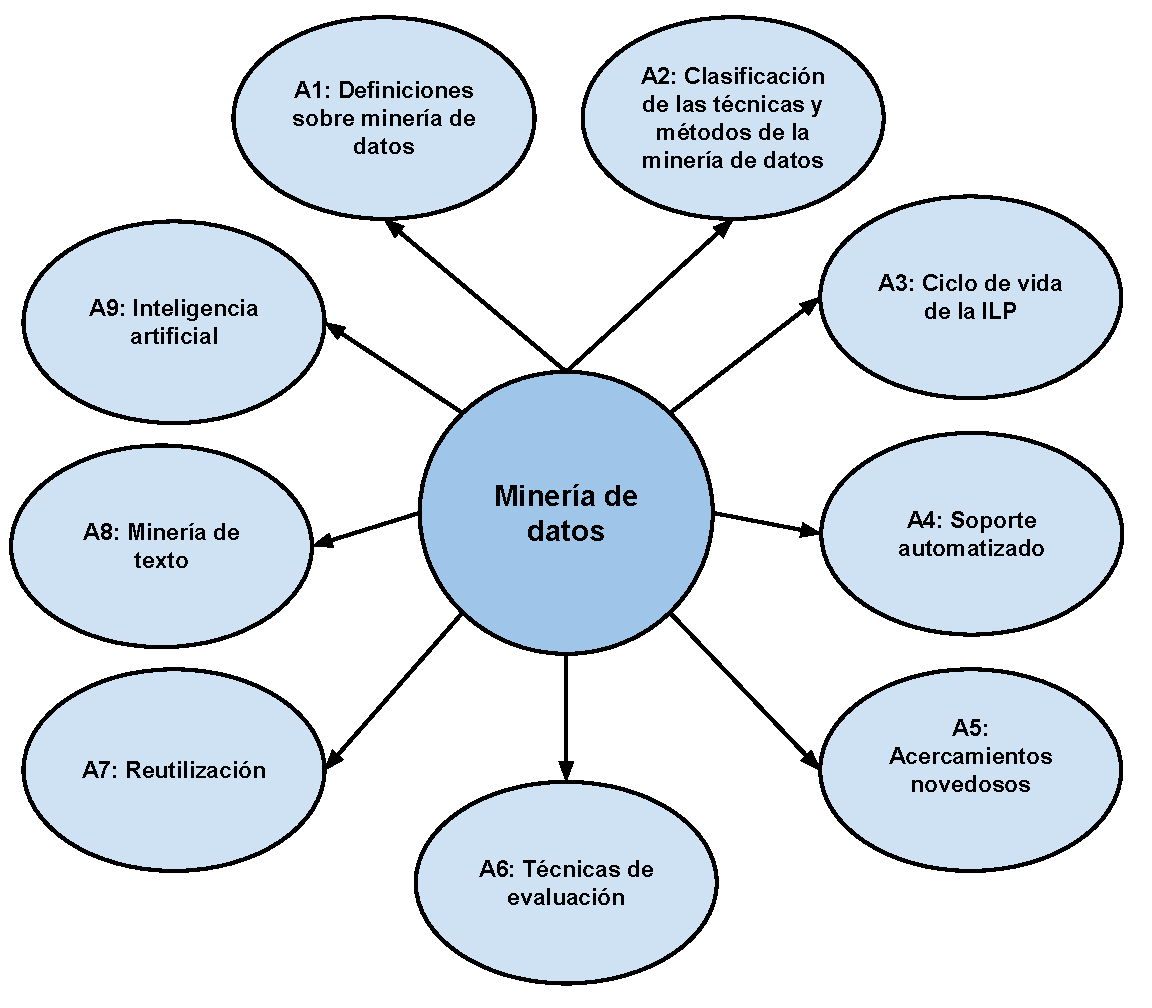
\includegraphics[width=0.825\textwidth]{framework}
    \caption{Marco de trabajo propuesto en la revisión de documentos.}
    \label{framework}
\end{figure}

\begin{description}

\item[Aspecto 1. Definiciones sobre minería de datos:]La MD es el proceso mediante el cual, haciendo uso de diferentes técnicas, se pretende encontrar patrones y relaciones en grandes cantidades de datos\cite{Izenman2006}; este aspecto, sin embargo, se centró en la definición de las técnicas de MD en el proceso de ILP que pudieran ser usadas para crear modelos de características.

\item[Aspecto 2. Clasificación de las técnicas y métodos de la minería de datos:] En este aspecto se realizaron definiciones de algunos criterios ilustrados por Hastie, T. \textit{et al.} \cite{Hastie2009} y Caruana R. \textit{et al.} \cite{Caruana2006} para comparar y extraer la información sobre las técnicas más apropiadas para desarrollar este estudio.

\item[Aspecto 3. Ciclo de vida de la ingeniería de líneas de producto:] En este aspecto se abordó el tema del ciclo de vida de la ILP como un proceso cuyo objetivo es crear grupos de productos que compartan ciertas características que logren satisfacer determinados nichos de mercado \cite{VanDerLinden2007}, teniendo en consideración la creación de productos personalizados de forma masiva.


\item[Aspecto 4. Soporte automatizado:] Dentro de la ILP es muy común representar un producto en la notación de MC teniendo en cuenta determinadas características y relaciones \cite{Benavides2010}. El propósito de este aspecto fue evidenciar la pertinencia de los MC dentro de los modelos de variabilidad, explicando el desarrollo incremental de los mismos y su mantenimiento automatizado a través del tiempo. 

\item[Aspecto 5. Acercamientos novedosos] En este aspecto se identificaron los métodos más utilizados y los trabajos más novedosos en el área de la MD.

\item[Aspecto 6. Técnicas de evaluación:] Debido a que las técnicas de MD son evaluadas teniendo en cuenta su ajuste a los datos de prueba, este aspecto propuso identificar y exponer los métodos de evaluación de las técnicas de MD considerando el tipo de datos, el contexto y el dominio. Con el propósito de adoptar un método de evaluación.

\item[Aspecto 7. Reutilización:] En este aspecto se identificaron los elementos reusables de los códigos utilizados en los diferentes enfoques de la MD, los conceptos involucrados y sus productos.

\item[Aspecto 8. Minería de texto:]  Este aspecto hizo hincapié en las herramientas o las diferentes técnicas de agrupamiento y su aplicación en grandes cantidades de datos. Desde el punto de vista de la construcción de MC, el interés consistió en revisar todas aquellas técnicas de agrupamiento que usaran árboles como estructuras jerárquicas.


\item[Aspecto 9. Inteligencia artificial:] Algunas técnicas de la MD son no supervisadas y bordean el tema de la inteligencia artificial. Con el propósito de cubrir la mayoría de documentos encontrados en el MSL, este aspecto se encargó de incluir el tema de la inteligencia artificial dentro del estudio.
\end{description}



La meta principal de esta sección fue establecer las preguntas de investigación que permitieran la clasificación de la literatura respecto a las técnicas de MD y la ILP utilizados en cualquier contexto. 
Para esto se establecieron preguntas basadas en metas más pequeñas que pretendieron orientar la búsqueda hacia las publicaciones que específicamente  usaron las técnicas de MD en el proceso de ILP .

Las metas en las que se basó la búsqueda se enumeran a continuación:

\subsubsection{Meta 1}
Obtener publicaciones con información sobre las técnicas de MD en el proceso de ILP. Las preguntas propuestas para el cumplimiento de esta meta se muestran en la Tabla \ref{tablag1}.

% --------------------------------------------- Tabla 1
\begin{longtable}{|c|p{7cm}|p{7cm}|}
\caption{Preguntas que apuntan a obtener las publicaciones con las técnicas de minería de datos en el proceso de ingeniería de líneas de producto.}\label{tablag1}\\
\hline
\textbf{ID} & \textbf{Pregunta de investigación} & \textbf{Motivación} \\
\hline
\endfirsthead
\multicolumn{3}{c}%
{\tablename\ \thetable\ -- \textit{Continuación de la página anterior}} \\
\hline
\textbf{ID} & \textbf{Pregunta de investigación} & \textbf{Motivación} \\
\hline
\endhead
\hline \multicolumn{3}{r}{\textit{Continúa en la siguiente página}} \\
\endfoot
\hline
\endlastfoot
RQ1 & ¿Cómo están distribuidos los estudios en el tiempo? & Representar la tendencia que ha tenido el trabajo de investigación en el tiempo. \tabularnewline \hline
RQ2 & ¿Qué tipo de documentos hablan del papel de la MD en la ILP? & Para los nuevos investigadores es interesante conocer cuáles son las revistas, conferencias, talleres o títulos de publicación que son protagonistas y abarcan la mayoría de los documentos. \tabularnewline \hline
RQ3 & ¿Qué distribución geográfica o cuáles autores son los más representativos en el presente estudio? & Con el propósito de considerar los grupos de investigación y las regiones interesantes para construir alianzas estratégicas y futuros trabajos.\tabularnewline \hline
RQ4 & ¿Qué categoría o escalafón de investigación tienen asignados los documentos encontrados en nuestro estudio? & Conociendo la categoría o el escalafón se puede establecer un grado de madurez en el tema de investigación como lo propone Wieringa, R. \textit{et al.} \cite{Wieringa2006}.\tabularnewline \hline
\end{longtable}

\subsubsection{Meta 2}
Identificar y caracterizar las técnicas de MD utilizadas en el proceso de ILP. Las preguntas propuestas para el cumplimiento de esta meta se muestran en la Tabla \ref{tablag2}.

% --------------------------------------------- Tabla 2
\begin{longtable}{|c|p{7cm}|p{7cm}|}
\caption{Preguntas que apuntan a identificar y caracterizar las técnicas de minería de datos usadas en el proceso de la ingeniería de líneas de producto.}\label{tablag2}\\
\hline
\textbf{ID} & \textbf{Pregunta de investigación} & \textbf{Motivación} \\
\hline
\endfirsthead
\multicolumn{3}{c}%
{\tablename\ \thetable\ -- \textit{Continuación de la página anterior}} \\
\hline
\textbf{ID} & \textbf{Pregunta de investigación} & \textbf{Motivación} \\
\hline
\endhead
\hline \multicolumn{3}{r}{\textit{Continúa en la siguiente página}} \\
\endfoot
\hline
\endlastfoot
RQ5 & ¿Qué algoritmos o técnicas son usadas en le ciclo de vida de la ILP para crear MC? & Identificar las técnicas apropiadas y los algoritmos para crear MC. \tabularnewline \hline
RQ6 & ¿Qué técnicas de la MD son usadas en el campo de la ILP? & Entender para qué se esta usando la MD en ILP con el fin de tener un entendimiento de su uso. \tabularnewline \hline
RQ7 & ¿Qué contexto de dominio está implementando MD e ILP? & Con el propósito de considerar las empresas y los sectores de la industria que pueden ser interesantes en la construcción de alianzas estratégicas y futuros trabajos.\tabularnewline \hline
RQ8 & ¿Cómo están definidas las técnicas de MD encontradas en los documentos? & Es importante la identificación de los procedimientos y los cálculos que se utilizan en las técnicas de MD.\tabularnewline \hline
RQ9 & ¿En cuál etapa del ciclo de vida de la ILP se usa la MD? & Asignar las técnicas encontradas a una etapa dentro del ciclo de vida de la ILP puede ser un marco de trabajo adecuado. \tabularnewline \hline
RQ10 & ¿Qué tipo de productos se han derivado del uso de las técnicas de MD en la ILP? & Es importante conocer qué se obtiene después de aplicar las técnicas de MD en las diferentes etapas del ciclo de vida de la ILP. \tabularnewline \hline
\end{longtable}

\subsubsection{Meta 3} 
Evaluar las técnicas de MD encontradas considerando la automatización de los MC. Las preguntas propuestas para el cumplimiento de esta meta se muestran en la Tabla \ref{tablag3}.

% --------------------------------------------- Tabla 3
\begin{longtable}{|c|p{7cm}|p{7cm}|}
\caption{Preguntas que apuntan a evaluar las técnicas de minería de datos encontradas, considerando la creación automática de los modelos de características.}\label{tablag3}\\
\hline
\textbf{ID} & \textbf{Pregunta de investigación} & \textbf{Motivación} \\
\hline
\endfirsthead
\multicolumn{3}{c}%
{\tablename\ \thetable\ -- \textit{Continuación de la página anterior}} \\
\hline
\textbf{ID} & \textbf{Pregunta de investigación} & \textbf{Motivación} \\
\hline
\endhead
\hline \multicolumn{3}{r}{\textit{Continúa en la siguiente página}} \\
\endfoot
\hline
\endlastfoot
RQ11 & ¿Cómo se puede validar el uso correcto de las técnicas de MD en ILP? & Con los enfoques de MD que propone Hastie, T. \textit{et al.} \cite{Hastie2009}  se puede considerar que las técnicas de MD están siendo aplicadas o usadas para el propósito que fueron diseñadas. \tabularnewline \hline
RQ12 & ¿Los estudios encontrados en la literatura apoyan la automatización de técnicas de MD? & Caracterizar la aplicabilidad de las técnicas de MD considerando su replicabilidad y automatización. \tabularnewline \hline
\end{longtable}

\subsubsection{Meta 4}
Identificar enfoques de mejoras y nuevos enfoques en técnicas de MD utilizadas en la ILP. Las preguntas propuestas para el cumplimiento de esta meta se muestran en la Tabla \ref{tablag4}.


% --------------------------------------------- Tabla 4
\begin{longtable}{|c|p{7cm}|p{7cm}|}
\caption{Preguntas que apuntan a identificar las mejoras y los enfoques novedosos en las técnicas de minería de datos usadas en la ingeniería de líneas de producto.}\label{tablag4}\\
\hline
\textbf{ID} & \textbf{Pregunta de investigación} & \textbf{Motivación} \\
\hline
\endfirsthead
\multicolumn{3}{c}%
{\tablename\ \thetable\ -- \textit{Continuación de la página anterior}} \\
\hline
\textbf{ID} & \textbf{Pregunta de investigación} & \textbf{Motivación} \\
\hline
\endhead
\hline \multicolumn{3}{r}{\textit{Continúa en la siguiente página}} \\
\endfoot
\hline
\endlastfoot
RQ13 & ¿Qué técnicas de MD pueden ser explotadas en la ILP? & Identificar las técnicas que son más importantes en el tema de interés. \tabularnewline \hline
RQ14 & ¿Entre los documentos encontrados son evidentes las propuestas innovadoras en la ILP? & Como una percepción subjetiva, realmente es enriquecedor para la investigación futura saber cuáles son las tendencias más atractivas. \tabularnewline \hline
\end{longtable}
 
\subsection{Estrategia de Búsqueda}

En el presente MSL como paso inicial se hizo uso de la búsqueda manual y la búsqueda automática, acompañada de un proceso de bola de nieve incremental desde adelante hacia atrás \textit{(backwards snowballing process)}\cite{Wohlin2014}, en el cual se miraron los títulos de los documentos, luego los resúmenes y finalmente, para completar el proceso de búsqueda, se buscaron documentos similares en las referencias y en los lugares de publicación.

\subsubsection{El estándar \textit{Quasi-Gold}}

Zhang, H. \textit{et al.} \cite{Zhang2011} propuso un enfoque para identificar los estudios pertinentes en la ingeniería de software mediante una revisión sistemática de la literatura, dicho enfoque está ilustrado en la Figura \ref{quasigold}. 
\begin{figure}[h]
    \centering
    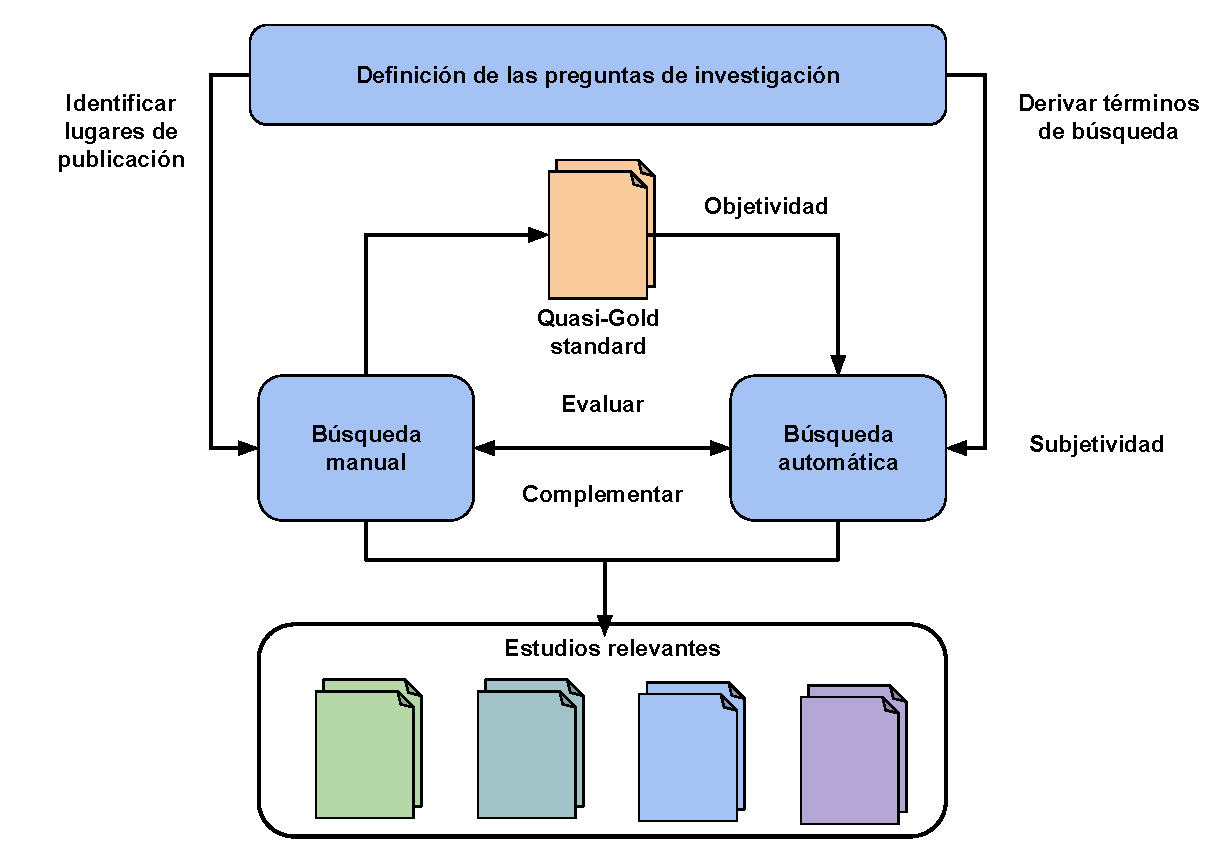
\includegraphics[width=0.7\textwidth]{quasigold}
    \caption{Estrategia de búsqueda propuesta por Zhang, H. \textit{et al.} para identificar los estudios pertinentes en ingeniería de software \cite{Zhang2011}.}
    \label{quasigold}
\end{figure}

Los anteriores conceptos fueron tomados en consideración teniendo en cuenta que un \textit{gold standard} representa, con la mayor exactitud posible, el conjunto conocido de los estudios primarios identificados en una colección de acuerdo con las preguntas de investigación propuestas en una revisión sistemática de literatura. De esta forma, una estrategia de búsqueda perfecta capturaría, exactamente, el \textit{gold standard} sin ningún resultado irrelevante. En consecuencia con lo anterior, Zhang, H. \textit{et al.} introduce el término \textit{quasi-gold estandard (QGS)} para obtener e identificar los estudios pertinentes en la ingeniería de software. Un QGS es un conjunto de estudios conocidos que son encontrados con una búsqueda manual en fuentes relacionadas (donde fueron publicados) durante un periodo de tiempo determinado. El QGS puede considerarse como un \textit{gold standar} en las condiciones en que estas restricciones (fuentes y tiempo) son aplicadas.
\\
Los QGS son útiles para hacer un método más objetivo con el fin de planificar y probar cadenas de búsqueda manuales y automáticas. La idea principal es evitar perder estudios relevantes en la estrategia de búsqueda, por tanto los resultados de las búsquedas manuales y automáticas se comparan con el QGS para calcular la sensibilidad y precisión de los resultados de la búsqueda. Es deseable obtener una alta sensibilidad en lugar de una alta precisión, dado que, una alta sensibilidad significa que se abarcan mas estudios. La sensibilidad por encima del 80\% es óptima para los mejores resultados, pero los resultados entre el 70\% y el 80\% también son aceptables según Zhang, H. \textit{et al.} \cite{Zhang2011}. Adicional al QGS, se utilizó otro método para ampliar la cobertura de la búsqueda y encontrar otros estudios pertinentes, este método se llama \textit{snowballing} \cite{Wohlin2014}, y consistió en utilizar la lista de referencias de un documento o las citas del documento para identificar estudios adicionales sobre el tema. Hay dos maneras de hacer \textit{snowballing}: \textit{snowballing} hacia atrás y \textit{snowballing} hacia adelante. En el presente proyecto se realizó \textit{snowballing} hacia atrás, lo cual consistió en utilizar la lista de referencias de los trabajos que ya habían sido seleccionado para obtener otros estudios relevantes sobre el tema. 

\subsubsection{Criterios de exclusión e inclusión }

Con el fin de realizar una cuidadosa selección de los estudios pertinentes, los documentos obtenidos deben ser verificados, primero, con criterios de exclusión; si un documento cumple con alguno de los criterios de exclusión, entonces será excluido. Los trabajos restantes se verifican con todos los criterios de inclusión para que sean aceptados.


\paragraph {Criterios de Exclusión:}
\begin{itemize}
\item \textbf{\textit{CE1: }} Documentos como reportes técnicos, lecciones aprendidas, borradores, estudios que describen eventos, afiches o pósteres y trabajos sin publicar que presenten MC.
\item \textbf{\textit{CE2: }} Documentos como artículos de opinión \textit{(Opinion articles or position papers)}.
\item \textbf{\textit{CE3: }} Documentos que no expliquen el uso de los métodos propuestos por la MD.
\item \textbf{\textit{CE4: }} Documentos que presenten MC, pero que no estén aplicados a la ILP.
\end{itemize}

\paragraph {Criterios de Inclusión:}
\begin{itemize}
	\item \textbf{\textit{CI1: }} Documentos (artículos, actas o memorias en conferencias, capítulos de libros o reportes de investigación) que presenten MC.
	\item \textbf{\textit{CI2: }} Documentos que presenten MC en el proceso de ILP.
	\item \textbf{\textit{CI3: }} Documentos que fueron publicados preferiblemente durante la última década del siglo XXI. %Documentos que fueron publicados en el siglo XXI, preferiblemente durante la última década.
	\item \textbf{\textit{CI4: }} Documentos que fueron publicados por profesores o personajes destacados.
\end{itemize}

\subsection{Escaneo de artículos}

Para seleccionar los trabajos pertinentes, se siguió el proceso descrito a continuación, el cual consta de tres etapas:

\begin{itemize}
\item Se realizó una búsqueda manual, utilizando los lugares de publicación que se enumeran . La búsqueda manual es útil para mejorar las cadenas de búsqueda utilizadas en la búsqueda automatizada y el QGS.
\item Se realizó una búsqueda automatizada, mediante el uso de los motores de búsqueda enumerados en la sección siguiente sección.
\item Finalmente, el proceso de \textit{Snowballing} en cada una de las primeras etapas, se realizó en tres rondas:
\begin{itemize}
\item Selección de trabajos según su título y palabras clave, utilizando los criterios de inclusión.
\item Selección de trabajos de acuerdo a su resumen de los trabajos seleccionados en la primera ronda. Aquí se utilizaron tanto los criterios de inclusión como los criterios de exclusión.
\item Selección del conjunto definitivo de trabajos revisando su texto completo utilizando todos los criterios de inclusión y exclusión.
\end{itemize}
\end{itemize}

\subsubsection{Tratamiento a los Documentos Repetidos}

Un documento duplicado es uno que se recupera de varias fuentes de búsqueda (es decir, bibliotecas digitales y lugares de publicación) por lo que se tiene más de una copia de la misma. El conjunto final de estudios pertinentes no debe incluir todas las copias de un documento duplicado. En consecuencia, los documentos duplicados se purgarán de modo que las copias adicionales se excluyan comparando la búsqueda manual y la búsqueda automática. Se llaman estudios repetidos a los artículos sobre el mismo estudio que se publican en varios lugares. Los estudios repetidos pueden contener los mismos autores, una combinación de los nombres del autor o la lista de autores con algunas variaciones. 

\subsubsection{Búsqueda Manual}\label{manual}

Antes de hacer una búsqueda automatizada, debe realizarse una búsqueda manual. La búsqueda manual se utiliza para identificar los estudios pertinentes. También contribuye a la elaboración del \textit{QGS} \cite{Zhang2011}. Este proceso consiste en una navegación manual de los lugares de publicación relevantes presentados a continuación.
Antes de presentar la búsqueda automática y los sitios de búsqueda, estas dos búsquedas se apoya en estudios que bien pueden ser considerados como \textit{QGS} o contribuyen a la elaboración de este proceso, por lo tanto, se seleccionaron los siguientes  documentos: \cite{Wang2014, Santos2015, Salinesi2009a, Souag2015, Farias2016, Soares2014, Sepulveda2016, Eleuterio2015, Bakar2015a}  y se considera usar sus lugares de publicación y el de sus referencias para este trabajo de investigación.  

\paragraph{Artículos}

\begin{enumerate}

\item \textbf{\textit{Information Sciences}}
\item \textbf{\textit{IEEE Transactions on Software Engineering}}
\item \textbf{\textit{Empirical Software Engineering}}
\item \textbf{\textit{Applied Soft Computing}}
\item \textbf{\textit{ACM Computing Surveys}}
\end{enumerate}
\paragraph{Conferencias, Talleres y Memorias}
\begin{enumerate}

\item \textbf{\textit{International Software Product Line Conference}}
\item \textbf{\textit{International Conference on Information Technology}}
\item \textbf{\textit{International Workshop on Product LinE Approaches in Software Engineering (PLEASE)}}
\item \textbf{\textit{Proceedings of the International Conference on Software Product Line - SPLC}}
\item \textbf{\textit{Proceedings of the IEEE}}
\item \textbf{\textit{Proceedings of the Annual ACM Symposium on Applied Computing - SAC}}
\item \textbf{\textit{Proceedings of the international conference on Machine learning - ICML}}
\item \textbf{\textit{Proceedings of the International Conference on Software and System Process - ICSSP}}
\item \textbf{\textit{Proceedings of the International Symposium on Computers in Education - SIIE}}
\item \textbf{\textit{Proceedings of the International Conference on Evaluation and Assessment in Software Engineering - EASE}}
\item \textbf{\textit{Proceedings of the ACM SIGKDD international conference on Knowledge discovery and data mining - KDD}}
\item \textbf{\textit{Proceedings of the International Conference on Computer Systems and Technologies - CompSysTech}}
\item \textbf{\textit{Proceedings of the Euromicro Conference Series on Software Engineering and Advanced Applications - SEAA}}

\end{enumerate}

\subsubsection{Búsqueda Automática}
La búsqueda automática se basa en obtener estudios relevantes usando las librerías digitales, esto se realiza de acuerdo a unas cadenas de búsqueda que se adaptan de acuerdo al motor que usa cada una de las librerías digitales. Estas búsquedas son más efectivas que las manuales pero el rendimiento depende de la calidad de la cadena de búsqueda, la capacidad de los motores de búsqueda y la diversidad o la popularidad de los documentos pertenecientes a la materia. Para mejorar la búsqueda automática, se hizo uso de las bibliotecas digitales y los índices, que proveen un gran repositorio de documentos y valiosas fuentes de publicación. Para la búsqueda automática seleccionaremos dos bases de datos digitales \textit{Scopus} y \textit{Web of Science}. \textit{Scopus} es largamente usada por que contiene indexadas la mayoría de las editoriales importantes como \textit{Elsevier}, \textit{IEEE}, \textit{Springer}, \textit{Wiley-Blackwell}, entre otras. \textit{Web of Science} también es muy útil por \textit{Inspec}. La búsqueda automática se completó con los resultados obtenidos en \textit{Google Scholar}, \textit{Nature} y \textit{Science}.


\subsection{Análisis de palabras clave}
En este trabajo de investigación, sólo se definió la siguiente cadena de búsqueda basada en los estudios recomendados, las facetas  y el concejo del investigador principal, y se examinaron los resultados considerando todos los criterios de inclusión y el proceso de \textit{Snowballing and Screaning of papers}.
\textbf{\textit{
(“product line*” OR “product famil*” OR variability OR “product platform*”) AND (“data mining” OR “Artificial Intelligence” OR “clustering” ) AND (“feature*” OR variabili*  OR characteristic*)
}}

\subsection{Proceso de Extracción de Datos}
Para la extracción de datos se usó la siguiente tecnología: \textit{Excel and Google Sheets, Splunk Enterprise \& Mendeley Desktop} teniendo en cuenta la información asociada con cada meta del proyecto de investigación.


\section{Diseño del prototipo}
La ciencia puede ser considera como una actividad que contribuye al entendimiento de un fenómeno. El fenómeno en este proyecto de investigación parte de una serie de comportamientos que pueden entenderse como unos patrones y la posibilidad de clasificaros,  Con el objetivo de producir un artefacto(software) que no existía se consideró \textit{Design Science} \cite{Vaishnavi2013} como una estrategia para el desarrollo de la investigación, una publicación o una patente. El prototipo de esta investigación partirá de la construcción de los modelos de características considerando los datos públicos de \href{http://archive.ics.uci.edu/ml/datasets/Iris}{Iris} y luego los de RIPS.
En este proyecto de investigación se siguió la metodología propuesta por \cite{Vaishnavi2013} y se resumió el proceso en: adquisición de la información, diseño y elaboración, demostración y evaluación.
 
\subsection{Adquisición de la información}
Desde La Facultad Nacional de Salud Pública ``Héctor Abad Gómez" de la Universidad de Antioquia nos fue entregada una gran colección de datos pertenecientes a  Los Registros Individuales de Prestación de Servicios de Salud (RIPS), lo primero que se realizó fue guardar esta información y realizar un respaldo, posteriormente se seleccionaron los primero $66262$ datos correspondientes al $0.1\%$. Debido a que no se conto con los recursos computacionales suficientes para realizar el procesamiento sobre la totalidad de los datos. En esta etapa se llevo a cabo una revisión preliminar de la información y se establecieron los posibles factores y variables que pudieran ser estadisticamente significativos en la construcción de los modelos de características. 

\subsection{Diseño y elaboración}
Para la construcción de los modelos y los diseños se realizaron entregas en Gráficos vectorizados Redimensionables \textit{Scalable Vector Graphics (SVG)} exportados al Formato de Documentos Portable \textit{Portable Document Format (PDF)} mediante \textit{InkScape}. En cada entrega se iniciaba una discusión sobre los supuestos en el diseño del método, y debido a que era una etapa temprana del proyecto se buscaron resultados conceptuales que se ajustaran a los mejores paradigmas encontrados en la literatura. Ademas se realizaron preguntas sobre ¿qué tan efectivo es el modelo planteado?,¿Soporta operaciones de complejidad elevada?,¿que operaciones soporta?,¿és escalable?,¿Cuales son las salidas y entradas en cada una de las etapas del modelo? En cada sesión se afinó el diseño hasta tener los requisitos para el desarrollo.
\subsection{Demostración}
Esta etapa de la metodología llamada \textit{Desing Science}, se basó en demostraciones simples de las tecnologías, para tener pequeños artefatos, como en nuestro caso \textit{Code Snippets} pàra el desarrollo conceptual del modelo. Su utilizo el \textit{Hortonworks sandbox}, los datos RIPS y los datos de \href{http://archive.ics.uci.edu/ml/datasets/Iris}{Iris}, y con esta forma de trabajar se establecieron reglas, restricciones existentes en la tecnología y se definieron cuales partes del diseño era necesario afinar.
\subsection{Evaluación}
Para esta etapa en el \textit{Designe Science} se hicieron una serie de pruebas de cada parte del modelo propuesto, estas pequeñas pruebas llamadas \textit{micro-evaluations} establecieron las pruebas formales al modelo después de tener una versión estable. En esta etapa también se establecieron los criterios de evaluación, en nuestro caso probar el ajuste de los datos y realizar el contraste entre los modelos de características al final del proceso planteado en el modelo. 

\section{Implementación del prototipo(Caso de aplicación)}

Como primera etapa de este desarrollo se tuvo el reconocimiento de los datos. En donde La Facultad Nacional de Salud Publica "Héctor Abad Gómez" puso a disposición del Grupo de Investigación de Ingeniería y Tecnologías de las Organizaciones y de la Sociedad (ITOS) los Registros Individuales de Prestación de Servicios de Salud (RIPS).
Luego se descubrieron las características técnicas indispensables para la adquisición de la información dado el peso de los datos, el siguiente paso fue el preporcesamiento de los datos, para el cual fue indispensable que el dueño del negocio (la persona que tiene conocimiento del contexto y el dominio) acompañe y valide los resultados, para efectos del desarrollo inicial se tomaron aproximadamente los primero 600 mil registros de la base de datos (0.01\%)  mediate el comando \emph{split} en \textit{macOS Sierra}.
En el prepocesamiento de los datos se desarrolla un \textit{script} en \textit{python (numpy, pandas, sklearn)}. En este  \textit{Pytthon Script}  se tuvieron como insumo inicial los datos que el cliente obtiene tras hacer un vaciado a archivo desde la base de datos que fue facilitada y, su posterior división para efectos del caso de aplicación. El resultado del \textit{Pytthon Script}  son los datos limpios para aplicar correctamente el algoritmo de minería de datos.
Esta etapa se conoce en la literatura como \textit{ETL}, y es definido como el proceso de extraer, transformar y cargar los datos en un volumen mas grande o una infraestructura de datos distribuidos, con el fin de facilitar la operaciones de las técnicas de inteligencia de negocio, minería de datos, aprendizaje de maquina, metaheurísticas e inteligencia artificial en los datos estandarizados o normalizados.
La segunda etapa de este proceso fue la elección de las técnicas a usar sobre los datos preparados, se  tomo el bloque de datos siguientes como pruebas y el actual como los datos como aprendizaje y se considero una selección de los factores. Se continuo  con esta parte de la etapa con la ayuda de  Caruana \textit{et al.}\cite{Caruana2006} y Hastie \textit{et al.} \cite{Hastie2009}, fue necesario tener las habilidades y la experiencia suficiente en reconocer cual es la técnica mas apropiada en el descubrimiento de las características en los RIPS, cuidando sobre todo  la clasificación del tipo de variables y los meta datos. Para ilustrar esta etapa presentamos un algoritmo desarrollado en \textit{R (randomForest, MASS, rpart, caret)}, Este \textit{R - Script} tiene como salida la selección de las características que mas aportan a la suma de cuadrados de los datos.
 Para el desarrollo de la tercera y ultima etapa se realizo un \textit{Java POJO} mediante el reconocimiento de una semántica basada en la lógica relacional, que tenga en cuenta los modelos de analítica descriptiva que se pueden generar en el formato \textit{Predictive Model Markup Language (PMML)} y los Modelos de características desarrollados en el formato \textit{ Simple XML Feature Model format (SXFM)}, que finalmente con la salida del \textit{R - script} se dispondrán los datos en un orden y un formato en que cual, las técnicas de minería se conviertan en la entrada de los software de diseño asistidos por computadora \textit{Computer-aided design (CAD)}, que se utilizan en el desarrollo de los Modelos de Características. Para escalar la solución a el 100\% de los datos se propuso en el diseño del modelo una infraestructura de \textit{Big Data} que pueda soportar la gran cantidad de datos en las industrias actuales.
